\chapter{Synchronization}

\epigraph{When multithreading gets interesting}{Bhuvy}

Synchronization are a series of mechanisms to control what threads are allowed to perform what operation at a time.
Most of the time, the threads can progress without having to communicate, but every so often two or more threads may want to access a critical section.
A critical section is a section of code that can only be executed by one thread at a time, if the program is to function correctly.
If two threads (or processes) were to execute code inside the critical section at the same time, it is possible that program may no longer have correct behavior.

As we said in the previous chapter, race conditions happen when an operation touches a piece of memory at the same time as another thread.
If the memory location is only accessible by one thread (e.g.~automatic variable \keyword{i} below) then there is no possibility of a race condition and no Critical Section associated with \keyword{i}.
However the \keyword{sum} variable is a global variable and accessed by two threads. It is possible that two threads may attempt to increment the variable at the same time.

\begin{lstlisting}[language=C]
#include <stdio.h>
#include <pthread.h>
// Compile with -pthread

int sum = 0; //shared

void *countgold(void *param) {
    int i; //local to each thread
    for (i = 0; i < 10000000; i++) {
        sum += 1;
    }
    return NULL;
}

int main() {
    pthread_t tid1, tid2;
    pthread_create(&tid1, NULL, countgold, NULL);
    pthread_create(&tid2, NULL, countgold, NULL);
    
    //Wait for both threads to finish:
    pthread_join(tid1, NULL);
    pthread_join(tid2, NULL);
    
    printf("ARRRRG sum is %d\n", sum);
    return 0;
}
\end{lstlisting}

Typical output of the above code is \keyword{ARGGGH sum is <some number less than expected>} because there is a race condition.
The code does not stop two threads from reading-writing \keyword{sum} at the same time.
For example, both threads copy the current value of sum into CPU that runs each thread (let's pick 123).
Both threads increment one to their own copy.
Both threads write back the value (124).
If the threads had accessed the sum at different times then the count would have been 125.
A few of the possible different orderings are below.

Permittable Pattern
\begin{tabular}{ l | r }
  Thread 1 & Thread 2 \\ \hline
  Load Addr, Add 1 (i=1 locally) & ...  \\
  Store (i=1 globally) & ...  \\
  ... & Load Addr, Add 1 (i=2 locally)  \\
  ... & Store (i=2 globally)  \\
\end{tabular}

Partial Overlap
\begin{tabular}{ l | r }
Thread 1 & Thread 2 \\ \hline
Load Addr, Add 1 (i=1 locally) & ... \\
Store (i=1 globally) & Load Addr, Add 1 (i=1 locally) \\
... & Store (i=1 globally) \\
\end{tabular}

Full Overlap
\begin{tabular}{ l | r }
Thread 1 & Thread 2 \\ \hline
Load Addr, Add 1 (i=1 locally) & Load Addr, Add 1 (i=1 locally) \\
Store (i=1 globally) & Store (i=1 globally) \\
\end{tabular}

We would like the first pattern of the code being mutually exclusive.
Which leads us to our first synchronization primitive, a Mutex.

\section{Mutex}

To ensure only one thread at a time can access a global variable, use a mutex -- short for Mutual Exclusion.
If one thread is currently inside a critical section we would like another thread to wait until the first thread is complete.

\begin{lstlisting}[language=C]
pthread_mutex_t m = PTHREAD_MUTEX_INITIALIZER; // global variable
pthread_mutex_lock(&m); // start of Critical Section
// Critical section
pthread_mutex_unlock(&m); //end of Critical Section
\end{lstlisting}

\subsection{Mutex Lifetime}

There are a few ways of initializing a mutex.
You can use the macro \keyword{PTHREAD\_MUTEX\_INITIALIZER} only for global (`static') variables.
\keyword{m = PTHREAD\_MUTEX\_INITIALIZER} is equivalent to the more general purpose \keyword{pthread\_mutex\_init(&m,NULL)}.
The init version includes options to trade performance for additional error-checking and advanced sharing options.
You can also call the init function inside of a program for a mutex located on the heap.

\begin{lstlisting}[language=C]
pthread_mutex_t *lock = malloc(sizeof(pthread_mutex_t)); 
pthread_mutex_init(lock, NULL);
//later
pthread_mutex_destroy(lock);
free(lock);
\end{lstlisting}

Once we are finished with the mutex we should also call \keyword{pthread\_mutex\_destroy(&m)} too.
Note, you can only destroy an unlocked mutex.
Things to keep in mind about \keyword{init} and \keyword{destroy}

\begin{enumerate} 
\item Multiple threads init/destroy has undefined behavior  
\item Destroying a locked mutex has undefined behavior  
\item Basically try to keep to the pattern of one thread initializing a mutex and one and only one thread initializing a mutex.
\item Copying the bytes of the mutex to a new memory location and then using the copy is \emph{not} supported. To reference a mutex, you have to have a pointer to that memory address.
\end{enumerate}

\subsection{Mutex Gotchas}

Mutexes do not lock variables.
A mutex is not that smart - it works with code, not data.
If I lock a mutex, the other threads will continue.
It's only when a thread attempts to lock a mutex that is already locked, will the thread have to wait.
As soon as the original thread unlocks the mutex, the second (waiting) thread will acquire the lock and be able to continue.
The following code creates a mutex that does effectively nothing.

\begin{lstlisting}[language=C]
int a;
pthread_mutex_t m1 = PTHREAD_MUTEX_INITIALIZER,
                 m2 = = PTHREAD_MUTEX_INITIALIZER;
// later
// Thread 1
pthread_mutex_lock(&m1);
a++;
pthread_mutex_unlock(&m1);

// Thread 2
pthread_mutex_lock(&m2);
a++;
pthread_mutex_unlock(&m2);
\end{lstlisting}

You can create mutex before fork-ing - however the child and parent process will not share virtual memory and each one will have a mutex independent of the other.
Advanced note: There are advanced options using shared memory that allow a child and parent to share a mutex if it's created with the correct options and uses a shared memory segment.
See \href{http://stackoverflow.com/questions/19172541/procs-fork-and-mutexes}{stackoverflow example}

As some other notes, the thread that locks a mutex is the only thread that can unlock it.
Each program can have multiple mutex locks, usually one lock per data structure.
If you only have one lock, then they may be significant contention for the lock between two threads that was unnecessary.
For example if two threads were updating two different counters, it might not be necessary to use the same lock.
However, simply creating many locks is insufficient: It's important to be able to reason about critical sections e.g.~it's important that one thread can't read two data structures while they are being updated and temporarily in an inconsistent state.
There is a small amount of overhead of calling \keyword{pthread\_mutex\_lock} and \keyword{pthread\_mutex\_unlock}.
However, this is the price you pay for correctly functioning programs!

\subsection{Simplest complete example}

Here is a complete example

\begin{lstlisting}[language=C]
#include <stdio.h>
#include <pthread.h>

// Compile with -pthread
// Create a mutex this ready to be locked!
pthread_mutex_t m = PTHREAD_MUTEX_INITIALIZER;

int sum = 0;

void *countgold(void *param) {
    int i;
    
    //Same thread that locks the mutex must unlock it
    //Critical section is just 'sum += 1'
    //However locking and unlocking a million times
    //has significant overhead
    
    pthread_mutex_lock(&m);

    // Other threads that call lock will have to wait until we call unlock

    for (i = 0; i < 10000000; i++) {
        sum += 1;
    }
    pthread_mutex_unlock(&m);
    return NULL;
}

int main() {
    pthread_t tid1, tid2;
    pthread_create(&tid1, NULL, countgold, NULL);
    pthread_create(&tid2, NULL, countgold, NULL);

    pthread_join(tid1, NULL);
    pthread_join(tid2, NULL);

    printf("ARRRRG sum is %d\n", sum);
    return 0;
}
\end{lstlisting}

In the code above, the thread gets the lock to the counting house before entering.
The critical section is only the \keyword{sum+=1} so the following version is also correct.

\begin{lstlisting}[language=C]
    for (i = 0; i < 10000000; i++) {
        pthread_mutex_lock(&m);
        sum += 1;
        pthread_mutex_unlock(&m);
    }
    return NULL;
}
\end{lstlisting}

This process runs slower because we lock and unlock the mutex a million times, which is expensive - at least compared with incrementing a variable.
In this simple example, we didn't really need threads - we could have added up twice!
A faster multi-thread example would be to add one million using an automatic (local) variable and only then adding it to a shared total after the calculation loop has finished:

\begin{lstlisting}[language=C]
    int local = 0;
    for (i = 0; i < 10000000; i++) {
       local += 1;
    }

    pthread_mutex_lock(&m);
    sum += local;
    pthread_mutex_unlock(&m);

    return NULL;
}
\end{lstlisting}

If I forget to unlock, you get deadlock!
We will talk about deadlock a little bit later but what is the problem with this loop if called by multiple threads.

\begin{lstlisting}[language=C]
while(not_stop){
    //stdin may not be thread safe
    pthread_mutex_lock(&m);
    char *line = getline(...);
    if(rand() % 2) { /* randomly skip lines */
         continue;
    }
    pthread_mutex_unlock(&m);
    
    process_line(line);
}
\end{lstlisting}

Other possible problems with synchronization.

\begin{itemize}
\tightlist
\item
  Not unlocking a mutex due to an early return during an error condition
\item
  Resource leak (not calling \keyword{pthread\_mutex\_destroy})
\item
  Using an unitialized mutex or using a mutex that has already been destroyed
\item
  Locking a mutex twice on a thread without unlocking first
\item
  Deadlock
\end{itemize}

\subsection{Mutex Implementation}

An incorrect implementation is shown below.
The \keyword{unlock} function simply unlocks the mutex and returns.
The lock function first checks to see if the lock is already locked.
If it is currently locked, it will keep checking again until another thread has unlocked the mutex.

\begin{lstlisting}[language=C]
// Version 1 (Incorrect!)

void lock(mutex_t *m) {
  while(m->locked) { /*Locked? Nevermind - just loop and check again!*/ }

  m->locked = 1;
}

void unlock(mutex_t *m) {
  m->locked = 0;
}
\end{lstlisting}

Version 1 uses `busy-waiting' (unnecessarily wasting CPU resources) however there is a more serious problem: We have a race-condition! If two threads both called \keyword{lock} concurrently it is possible that both threads would read \keyword{m\_locked} as zero.
Thus both threads would believe they have exclusive access to the lock and both threads will continue. Ooops!

We might attempt to reduce the CPU overhead a little by calling \keyword{pthread\_yield()} inside the loop - pthread\_yield suggests to the operating system that the thread does not use the CPU for a short while, so the CPU may be assigned to threads that are waiting to run.
But does not fix the race-condition. We need a better implementation - can you work how to prevent the race-condition?


\subsection{Extra: Implementing a Mutex with hardware}

We can use C11 Atomics to do that perfectly!
A complete solution is detailed here.
This is a spinlock mutex, \href{https://locklessinc.com/articles/mutex_cv_futex/}{futex} implementations can be found online.

\begin{lstlisting}[language=C]
typedef struct mutex_{
    atomic_int_least8_t lock;
    pthread_t owner;
} mutex;

#define UNLOCKED 0
#define LOCKED 1
#define UNASSIGNED_OWNER 0

int mutex_init(mutex* mtx){
    if(!mtx){
        return 0;
    }
    atomic_init(&mtx->lock, UNLOCKED); // Not thread safe the user has to take care of this
    mtx->owner = UNASSIGNED_OWNER;
    return 1;
}
\end{lstlisting}

This is the initialization code, nothing fancy here.
We set the state of the mutex to unlocked and set the owner to locked.

\begin{lstlisting}[language=C]
int mutex_lock(mutex* mtx){
    int_least8_t zero = UNLOCKED;
    while(!atomic_compare_exchange_weak_explicit
            (&mtx->lock, 
             &zero, 
             LOCKED,
             memory_order_relaxed,
             memory_order_relaxed)){
        zero = UNLOCKED;
        sched_yield(); // Use system calls for scheduling speed
    }
    // We have the lock now
    mtx->owner = pthread_self();
    return 1;
}
\end{lstlisting}

What does this code do? Well to start it it initializes a variable that we will keep as the unlocked state.
\href{https://en.wikipedia.org/wiki/Compare-and-swap}{Atomic Compare and Exchange} is an instruction supported by most modern architectures (on x86 it's \keyword{lock cmpxchg}).
The pseudocode for this operation looks like this

\begin{lstlisting}[language=C]
int atomic_compare_exchange_pseudo(int* addr1, int* addr2, int val){
    if(*addr1 == *addr2){
        *addr1 = val;
        return 1;
    }else{
        *addr2 = *addr1;
        return 0;
    }
}
\end{lstlisting}

Except it is all done \emph{atomically} meaning in one uninterruptible operation.
What does the \emph{weak} part mean?
Well atomic instructions are prone to \textbf{spurious failures} meaning that there are two versions to these atomic functions a \emph{strong} and a \emph{weak} part, strong guarantees the success or failure while weak may fail.
We are using weak because weak is faster, and we are in a loop!
That means we are okay if it fails a little bit more often because we will just keep spinning around anyway.

Inside the while loop, we have failed to grab the lock!
We reset zero to unlocked and sleep for a little while.
When we wake up we try to grab the lock again.
Once we successfully swap, we are in the critical section!
We set the mutex's owner to the current thread for the unlock method and return successful.

How does this guarantee mutual exclusion, when working with atomics we are not entirely sure!
But in this simple example we can because the thread that is able to successfully expect the lock to be UNLOCKED (0) and swap it to a LOCKED (1) state is considered the winner.
How do we implement unlock?

What is this memory order business?
We were talking about memory fences earlier, here it is!
We won't go into detail because it is outside the scope of this course but not the scope of \href{https://gcc.gnu.org/wiki/Atomic/GCCMM/AtomicSync}{this article}.

\begin{lstlisting}[language=C]
int mutex_unlock(mutex* mtx){
    if(unlikely(pthread_self() != mtx->owner)){
        return 0; //You can't unlock a mutex if you aren't the owner
    }
    int_least8_t one = 1;
    //Critical section ends after this atomic
    mtx->owner = UNASSIGNED_OWNER;
    if(!atomic_compare_exchange_strong_explicit(
                &mtx->lock, 
                &one, 
                UNLOCKED,
                memory_order_relaxed,
                memory_order_relaxed)){
        //The mutex was never locked in the first place
        return 0;
    }
    return 1;
}
\end{lstlisting}

To satisfy the api, you can't unlock the mutex unless you are the one who owns it.
Then we unassign the mutex owner, because critical section is over after the atomic.
We want a strong exchange because we don't want to block (pthread\_mutex\_unlock doesn't block).
We expect the mutex to be locked, and we swap it to unlock.
If the swap was successful, we unlocked the mutex.
If the swap wasn't, that means that the mutex was UNLOCKED and we tried to switch it from UNLOCKED to UNLOCKED, preserving the non blocking of unlock.

\subsection{Semaphore}

Using a semaphore is as easy as creating a mutex.
First decide if the initial value should be zero or some other value (e.g.~the number of remaining spaces in an array).
Unlike pthread mutex there are not shortcuts to creating a semaphore - use \keyword{sem\_init}

\begin{lstlisting}[language=C]
#include <semaphore.h>

sem_t s;
int main() {
  sem_init(&s, 0, 10); // returns -1 (=FAILED) on OS X
  sem_wait(&s); // Could do this 10 times without blocking
  sem_post(&s); // Announce that we've finished (and one more resource item is available; increment count)
  sem_destroy(&s); // release resources of the semaphore
}
\end{lstlisting}

When using a semaphore, wait and post can be called from different threads!
Unlike a mutex, the increment and decrement can be from different threads.
This becomes especially useful if you want to use a semaphore to implement a mutex.
A mutex is a semaphore that always \keyword{waits} before it \keyword{posts}.
Some textbooks will refer to a mutex as a binary semaphore.
You do have to be careful to never add more than one to a semaphore or otherwise your mutex abstraction breaks.
That is usually why a mutex is used to implement a semaphore and vice versa.

\begin{itemize}
\item Initialize the semaphore with a count of one. 
\item Replace \keyword{pthread\_mutex\_lock} with \keyword{sem\_wait} 
\item Replace \keyword{pthread\_mutex\_unlock} with \keyword{sem\_post}
\end{itemize}

\begin{lstlisting}[language=C]
sem_t s;
sem_init(&s, 0, 1);

sem_wait(&s);
// Critical Section
sem_post(&s);
\end{lstlisting}

Also, keyword{sem\_post} is one of a handful of functions that can be correctly used inside a signal handler (\keyword{pthread\_mutex\_unlock} is not).
This means we can release a waiting thread which can now make all of the calls that we were not allowed to call inside the signal handler itself e.g. \keyword{printf}.

\begin{lstlisting}[language=C]
#include <stdio.h>
#include <pthread.h>
#include <signal.h>
#include <semaphore.h>
#include <unistd.h>

sem_t s;

void handler(int signal) {
    sem_post(&s); /* Release the Kraken! */
}

void *singsong(void *param) {
    sem_wait(&s);
    printf("I had to wait until your signal released me!\n");
}

int main() {
    int ok = sem_init(&s, 0, 0 /* Initial value of zero*/); 
    if (ok == -1) {
       perror("Could not create unnamed semaphore");
       return 1;
    }
    signal(SIGINT, handler); // Too simple! See Signals chapter

    pthread_t tid;
    pthread_create(&tid, NULL, singsong, NULL);
    pthread_exit(NULL); /* Process will exit when there are no more threads */
}
\end{lstlisting}

\section{Condition Variables}

Condition variables allow a set of threads to sleep until woken up.
You can wake up one thread or all threads that are sleeping.
If you only wake one thread then the operating system will decide which thread to wake up.
You don't wake threads directly instead you `signal' the condition variable, which then will wake up one (or all) threads that are sleeping inside the condition variable.

Condition variables are also generally used with a mutex and with a loop, so when woken up they have to check a condition in a critical section.
If you just need to be woken up not in a critical section, there are other ways to do this in POSIX.
Threads sleeping inside a condition variable are woken up by calling \keyword{pthread\_cond\_broadcast} (wake up all) or \keyword{pthread\_cond\_signal} (wake up one).
Note despite the function name, this has nothing to do with POSIX \keyword{signal}s!

Occasionally a waiting thread may appear to wake up for no reason (this is called a \emph{spurious wake}).
This is not an issue because you always use \keyword{wait} inside a loop that tests a condition that must be true to continue.

Why do spurious wakeups happen?
For performance. On multi-CPU systems it is possible that a race-condition could cause a wake-up (signal) request to be unnoticed.
The kernel may not detect this lost wake-up call but can detect when it might occur. To avoid the potential lost signal the thread is woken up so that the program code can test the condition again.

\begin{comment}

\subsection{Extra: Why do Condition Variables also need a mutex?}

Condition variables need a mutex for three reasons. The simplest to understand is that it prevents an early wakeup message (\keyword{signal} or \keyword{broadcast} functions) from being `lost.' Imagine the following sequence of events (time runs down the page) where the condition is satisfied \emph{just before} \keyword{pthread\_cond\_wait} is called. In this example the wake-up signal is lost!

Thread 1 \textbar{} Thread 2 -------------------------\textbar{}--------- \keyword{while( answer < 42) {} \textbar{} \textbar{} \keyword{answer++} \textbar{} \keyword{p\_cond\_signal(cv)} \keyword{p\_cond\_wait(cv,m)} \textbar{}

If both threads had locked a mutex, the signal can not be sent until \emph{after} \keyword{pthread\_cond\_wait(cv, m)} is called (which then internally unlocks the mutex)

A second common reason is that updating the program state (\keyword{answer} variable) typically requires mutual exclusion - for example multiple threads may be updating the value of \keyword{answer}.

A third and subtle reason is to satisfy real-time scheduling concerns which we only outline here: In a time-critical application, the waiting thread with the \emph{highest priority} should be allowed to continue first. To satisfy this requirement the mutex must also be locked before calling \keyword{pthread\_cond\_signal} or \keyword{pthread\_cond\_broadcast} . For the curious, a longer and historical discussion is \href{https://groups.google.com/forum/?hl=ky\#!msg/comp.programming.threads/wEUgPq541v8/ZByyyS8acqMJ}{here}.

\end{comment}

\subsection{Cond Wait Example}

The call \keyword{pthread\_cond\_wait} performs three actions: 

\begin{enumerate}
\item Unlock the mutex if given
\item Sleeps until \keyword{pthread\_cond\_signal} is called on the same condition variable) 
\item Before returning, locks the mutex if given
\end{enumerate}

Condition variables are \emph{always} used with a mutex lock.
Before calling \emph{wait}, the mutex lock must be locked and \emph{wait} must be wrapped with a loop.

\begin{lstlisting}[language=C]
pthread_cond_t cv;
pthread_mutex_t m;
int count;

// Initialize
pthread_cond_init(&cv, NULL);
pthread_mutex_init(&m, NULL);
count = 0;

pthread_mutex_lock(&m);
while (count < 10) {
   pthread_cond_wait(&cv, &m); 
  /* Remember that cond_wait unlocks the mutex before blocking (waiting)! */
  /* After unlocking, other threads can claim the mutex. */
  /* When this thread is later woken it will */
  /* re-lock the mutex before returning */
}
pthread_mutex_unlock(&m);

//later clean up with pthread_cond_destroy(&cv); and mutex_destroy 


// In another thread increment count:
while (1) {
  pthread_mutex_lock(&m);
  count++;
  pthread_cond_signal(&cv);
  /* Even though the other thread is woken up it cannot not return */
  /* from pthread_cond_wait until we have unlocked the mutex. This is */
  /* a good thing! In fact, it is usually the best practice to call */
  /* cond_signal or cond_broadcast before unlocking the mutex */
  pthread_mutex_unlock(&m);
}
\end{lstlisting}

\section{Thread Safe Data Structures}

Atomicity is when an operation is thread safe.
We have atomic instructions in hardware by providing the lock prefix
\begin{lstlisting}
lock ...
\end{lstlisting}
But atomicity also applies to higher orders of operations
We say a data structure operation if it happens all at once and successfully or not at all.

As such, we can use the tools in the previous section in order to make our data structures thread safe.
For the most part, we will be using mutexes because they carry more semantic meaning than a binary semaphore.
Note, this is just an introduction - writing high-performance thread-safe data structures requires its own book!
Take for example the following non thread-safe stack.

\begin{lstlisting}[language=C]
// A simple fixed-sized stack (version 1)
#define STACK_SIZE 20
int count;
double values[STACK_SIZE];

void push(double v) { 
    values[count++] = v; 
}

double pop() {
    return values[--count];
}

int is_empty() {
    return count == 0;
}
\end{lstlisting}

Version 1 of the stack is not thread-safe because if two threads call push or pop at the same time then the results or the stack can be inconsistent.
For example, imagine if two threads call pop at the same time then both threads may read the same value, both may read the original count value.

To turn this into a thread-safe data structure we need to identify the \emph{critical sections} of our code i.e.~which section(s) of the code must only have one thread at a time.
In the above example the \keyword{push},\keyword{pop} and \keyword{is\_empty} functions access the same variables (i.e.~memory) and all critical sections for the stack.
While \keyword{push} (and \keyword{pop}) is executing, the datastructure is an inconsistent state (for example the count may not have been written to, so may still contain the original value).
By wrapping these methods with a mutex we can ensure that only one thread at a time can update (or read) the stack. A candidate `solution' is shown below.
Is it correct? If not, how will it fail?

\begin{lstlisting}[language=C]
// An attempt at a thread-safe stack (version 2)
#define STACK_SIZE 20
int count;
double values[STACK_SIZE];

pthread_mutex_t m1 = PTHREAD_MUTEX_INITIALIZER;
pthread_mutex_t m2 = PTHREAD_MUTEX_INITIALIZER;

void push(double v) { 
    pthread_mutex_lock(&m1);
    values[count++] = v;
    pthread_mutex_unlock(&m1);
}

double pop() {
    pthread_mutex_lock(&m2);
    double v = values[--count];
    pthread_mutex_unlock(&m2);

    return v;
}

int is_empty() {
    pthread_mutex_lock(&m1);
    return count == 0;
    pthread_mutex_unlock(&m1);
}
\end{lstlisting}

Version 2 contains at least one error.
Take a moment to see if you can the error(s) and work out the consequence(s).

If three threads called \keyword{push()} at the same time the lock \keyword{m1} ensures that only one thread at time manipulates the stack (two threads will need to wait until the first thread completes (calls unlock), then a second thread will be allowed to continue into the critical section and finally the third thread will be allowed to continue once the second thread has finished).
A similar argument applies to concurrent calls (calls at the same time) to \keyword{pop}. However version 2 does not prevent push and pop from running at the same time because \keyword{push} and \keyword{pop} use two different mutex locks. The fix is simple in this case - use the same mutex lock for both the push and pop functions.

The code has a second error; \keyword{is\_empty} returns after the comparison and will not unlock the mutex.
However, the error would not be spotted immediately.
For example, suppose one thread calls \keyword{is\_empty} and a second thread later calls \keyword{push}.
This thread would mysteriously stop.
Using debugger you can discover that the thread is stuck at the lock() method inside the \keyword{push} method because the lock was never unlocked by the earlier \keyword{is\_empty} call.
Thus an oversight in one thread led to problems much later in time in an arbitrary other thread.

\begin{lstlisting}[language=C]
// An attempt at a thread-safe stack (version 3)
int count;
double values[count];
pthread_mutex_t m = PTHREAD_MUTEX_INITIALIZER;

void push(double v) { 
  pthread_mutex_lock(&m); 
  values[count++] = v;
  pthread_mutex_unlock(&m);
}
double pop() {
  pthread_mutex_lock(&m);
  double v = values[--count];
  pthread_mutex_unlock(&m);
  return v;
}
int is_empty() {
  pthread_mutex_lock(&m);
  int result = count == 0;
  pthread_mutex_unlock(&m);
  return result;
}
\end{lstlisting}

Version 3 is thread-safe.
We have ensured mutual exclusion for all of the critical sections.
There are a few things to note.

\begin{itemize}
\item \keyword{is\_empty} is thread-safe but its result may already be out-of date i.e.~the stack may no longer be empty by the time the thread gets the result!
  This is usually why in thread safe data structures, functions that return sizes are removed or depricated.
  \item There is no protection against underflow (popping on an empty stack) or overflow (pushing onto an already-full stack)
\end{itemize}

The last point can be fixed using counting semaphores. The implementation assumes a single stack. A more general purpose version might include the mutex as part of the memory struct and use \keyword{pthread\_mutex\_init} to initialize the mutex. For example,

\begin{lstlisting}[language=C]
// Support for multiple stacks (each one has a mutex)
typedef struct stack {
    int count;
    pthread_mutex_t m; 
    double *values;
} stack_t;

stack_t* stack_create(int capacity) {
    stack_t *result = malloc(sizeof(stack_t));
    result->count = 0;
    result->values = malloc(sizeof(double) * capacity);
    pthread_mutex_init(&result->m, NULL);
    return result;
}
void stack_destroy(stack_t *s) {
    free(s->values);
    pthread_mutex_destroy(&s->m);
    free(s);
}

// Warning no underflow or overflow checks!

void push(stack_t *s, double v) { 
    pthread_mutex_lock(&s->m); 
    s->values[(s->count)++] = v; 
    pthread_mutex_unlock(&s->m);
}

double pop(stack_t *s) { 
    pthread_mutex_lock(&s->m); 
    double v = s->values[--(s->count)]; 
    pthread_mutex_unlock(&s->m); 
    return v;
}

int is_empty(stack_t *s) { 
    pthread_mutex_lock(&s->m); 
    int result = s->count == 0; 
    pthread_mutex_unlock(&s->m);
    return result;
}

int main() {
    stack_t *s1 = stack_create(10 /* Max capacity*/);
    stack_t *s2 = stack_create(10);
    push(s1, 3.141);
    push(s2, pop(s1));
    stack_destroy(s2);
    stack_destroy(s1);
}
\end{lstlisting}

\subsection{Using semaphores}

We can also use a counting semaphore to keep track of how many spaces remain and another semaphore to keep to track the number of items in the stack. We will call these two semaphores `sremain' and `sitems'. Remember \keyword{sem\_wait} will wait if the semaphore's count has been decremented to zero (by another thread calling sem\_post).

\begin{lstlisting}[language=C]
// Sketch #1

sem_t sitems;
sem_t sremain;
void stack_init(){
  sem_init(&sitems, 0, 0);
  sem_init(&sremain, 0, 10);
}


double pop() {
  // Wait until there's at least one item
  sem_wait(&sitems);
  ...

void push(double v) {
  // Wait until there's at least one space
  sem_wait(&sremain);
  ...
}
\end{lstlisting}

Sketch \#2 has implemented the \keyword{post} too early. Another thread waiting in push can erroneously attempt to write into a full stack (and similarly a thread waiting in the pop() is allowed to continue too early).

\begin{lstlisting}[language=C]
// Sketch #2 (Error!)
double pop() {
  // Wait until there's at least one item
  sem_wait(&sitems);
  sem_post(&sremain); // error! wakes up pushing() thread too early
  return values[--count];
}
void push(double v) {
  // Wait until there's at least one space
  sem_wait(&sremain);
  sem_post(&sitems); // error! wakes up a popping() thread too early
  values[count++] = v;
}
\end{lstlisting}

Sketch 3 implements the correct semaphore logic but can you spot the error?

\begin{lstlisting}[language=C]
// Sketch #3 (Error!)
double pop() {
  // Wait until there's at least one item
  sem_wait(&sitems);
  double v= values[--count];
  sem_post(&sremain);
  return v;
}

void push(double v) {
  // Wait until there's at least one space
  sem_wait(&sremain);
  values[count++] = v;
  sem_post(&sitems); 
}
\end{lstlisting}

Sketch 3 correctly enforces buffer full and buffer empty conditions using semaphores.
However there is no \emph{mutual exclusion}: Two threads can be in the \emph{critical section} at the same time, which would corrupt the data structure (or least lead to data loss). The fix is to wrap a mutex around the critical section:

\begin{lstlisting}[language=C]
// Simple single stack - see above example on how to convert this into a multiple stacks.
// Also a robust POSIX implementation would check for EINTR and error codes of sem_wait.

// PTHREAD_MUTEX_INITIALIZER for statics (use pthread_mutex_init() for stack/heap memory)

pthread_mutex_t m= PTHREAD_MUTEX_INITIALIZER; 
int count = 0;
double values[10];
sem_t sitems, sremain;

void init() {
  sem_init(&sitems, 0, 0);
  sem_init(&sremains, 0, 10); // 10 spaces
}

double pop() {
  // Wait until there's at least one item
  sem_wait(&sitems);

  pthread_mutex_lock(&m); // CRITICAL SECTION
  double v= values[--count];
  pthread_mutex_unlock(&m);

  sem_post(&sremain); // Hey world, there's at least one space
  return v;
}

void push(double v) {
  // Wait until there's at least one space
  sem_wait(&sremain);

  pthread_mutex_lock(&m); // CRITICAL SECTION
  values[count++] = v;
  pthread_mutex_unlock(&m);

  sem_post(&sitems); // Hey world, there's at least one item
}
// Note a robust solution will need to check sem_wait's result for EINTR (more about this later)
\end{lstlisting}

\section{Candidate Solutions to the Critical Section}\label{candidate-solutions}

As already discussed, there are critical parts of our code that can only be executed by one thread at a time.
We describe this requirement as `mutual exclusion'; only one thread (or process) may have access to the shared resource.
In multi-threaded programs, we can wrap a critical section with mutex lock and unlock calls:

\begin{lstlisting}[language=C]
pthread_mutex_lock() - one thread allowed at a time! (others will have to wait here)
... Do Critical Section stuff here!
pthread_mutex_unlock() - let other waiting threads continue
\end{lstlisting}

How would we implement these lock and unlock calls?
Can we create an algorithm that assures mutual exclusion?

\begin{lstlisting}[language=C]
pthread_mutex_lock(p_mutex_t *m)     { while(m->lock) {}; m->lock = 1;}
pthread_mutex_unlock(p_mutex_t *m)   { m->lock = 0; }
\end{lstlisting}

At first glance, the code appears to work; if one thread attempts to locks the mutex, a later thread must wait until the lock is cleared. However this implementation \emph{does not satisfy Mutual Exclusion}. Let's take a close look at this `implementation' from the point of view of two threads running around the same time.

\todo{Thread ascii art or x86}

To simplify the discussion we consider only two threads. Note, these arguments work for threads and processes and the classic CS literature discusses these problem in terms of two processes that need exclusive access (i.e.~mutual exclusion) to a critical section or shared resource. Raising a flag represents a thread/process's intention to enter the critical section.

Remember that the psuedo-code outlined below is part of a larger program; the thread or process will typically need to enter the critical section many times during the lifetime of the process. So imagine each example as wrapped inside a loop where for a random amount of time the thread or process is working on something else.

Is there anything wrong with candidate solution described below?

\begin{lstlisting}
// Candidate #1
wait until your flag is lowered
raise my flag
// Do Critical Section stuff
lower my flag 
\end{lstlisting}

Answer: Candidate solution \#1 also suffers a race condition i.e.~it does not satisfy Mutual Exclusion because both threads/processes could read each other's flag value (=lowered) and continue.

This suggests we should raise the flag \emph{before} checking the other thread's flag - which is candidate solution \#2 below.

\begin{lstlisting}
// Candidate #2
raise my flag
wait until your flag is lowered
// Do Critical Section stuff
lower my flag 
\end{lstlisting}

Candidate \#2 satisfies mutual exclusion - it is impossible for two threads to be inside the critical section at the same time. However this code suffers from deadlock! Suppose two threads wish to enter the critical section at the same time:

\begin{tabular}{|l|c|c|}
Time & Thread 1 & Thread 2 \\ \hline
1 & Raise Flag & \\
2 & & Raise Flag \\
3 & Wait & Wait \\
\end{tabular}

Ooops both threads / processes are now waiting for the other one to lower their flags. Neither one will enter the critical section as both are now stuck forever! This suggests we should use a turn-based variable to try to resolve who should proceed.

\subsection{Turn-based solutions}\label{turn-based-solutions}

The following candidate solution \#3 uses a turn-based variable to politely allow one thread and then the other to continue

\begin{lstlisting}
// Candidate #3
wait until my turn is myid
// Do Critical Section stuff
turn = yourid
\end{lstlisting}

Candidate \#3 satisfies mutual exclusion (each thread or process gets exclusive access to the Critical Section), however both threads/processes must take a strict turn-based approach to using the critical section; i.e.~they are forced into an alternating critical section access pattern. For example, if thread 1 wishes to read a hashtable every millisecond but another thread writes to a hashtable every second, then the reading thread would have to wait another 999ms before being able to read from the hashtable again. This `solution' is not effective, because our threads should be able to make progress and enter the critical section if no other thread is currently in the critical section.

\subsection{Desired properties for solutions to the Critical Section Problem}

There are three main desirable properties that we desire in a solution the critical section problem

\begin{enumerate}
\item Mutual Exclusion - the thread/process gets exclusive access; others must wait until it exits the critical section.
\item Bounded Wait - if the thread/process has to wait, then it should only have to wait for a finite, amount of time (infinite waiting times are not allowed!). The exact definition of bounded wait is that there is an upper (non-infinite) bound on the number of times any other process can enter its critical section before the given process enters.
\item Progress - if no thread/process is inside the critical section, then the thread/process should be able to proceed (make progress) without having to wait.
\end{enumerate}

With these ideas in mind let's examine another candidate solution that uses a turn-based flag only if two threads both required access at the same time.

\subsection{Turn and Flag solutions}

Is the following a correct solution to CSP?

\begin{lstlisting}
\\ Candidate #4
raise my flag
if your flag is raised, wait until my turn
// Do Critical Section stuff
turn = yourid
lower my flag
\end{lstlisting}

One instructor and another CS faculty member initially thought so!
However, analyzing these solutions is tricky.
Even peer-reviewed papers on this specific subject contain incorrect solutions!
At first glance it appears to satisfy Mutual Exclusion, Bounded Wait and Progress: The turn-based flag is only used in the event of a tie (so Progress and Bounded Wait is allowed) and mutual exclusion appears to be satisfied.
Perhaps you can find a counter-example?

Candidate \#4 fails because a thread does not wait until the other thread lowers their flag.
After some thought (or inspiration) the following scenario can be created to demonstrate how Mutual Exclusion is not satisfied.

Imagine the first thread runs this code twice (so the the turn flag now points to the second thread).
While the first thread is still inside the Critical Section, the second thread arrives.
The second thread can immediately continue into the Critical Section!

\begin{tabular}{|l|l|l|l|}
Time & Turn & Thread \# 1 & Thread \# 2 \\ \hline
1 & 2 & Raise my flag & \\
2 & 2 & If your flag is raise, wait until my turn & Raise my flag \\
3 & 2 & // Do Critical Section Stuff & If your flag is raised, wait until my turn (TRUE!) \\
4 & 2 & // Do Critical Section Stuff & Do Critical Section Stuff - OOPS \\
\end{tabular}

\section{Working Solutions}\label{working-solutions}

\subsection{What is Peterson's solution?}\label{what-is-petersons-solution}

Peterson published his novel and surprisingly simple solution in a 2 page paper in 1981. A version of his algorithm is shown below that uses a shared variable \keyword{turn}:

\begin{lstlisting}
\\ Candidate #5
raise my flag
turn = your_id
wait until your flag is lowered and turn is yourid
// Do Critical Section stuff
lower my flag
\end{lstlisting}

This solution satisfies Mutual Exclusion, Bounded Wait and Progress.
If thread \#2 has set turn to 2 and is currently inside the critical section.
Thread \#1 arrives, \emph{sets the turn back to 1} and now waits until thread 2 lowers the flag.

Link to Peterson's original article pdf: \href{http://dl.acm.org/citation.cfm?id=945527}{G. L. Peterson: ``Myths About the Mutual Exclusion Problem'', Information Processing Letters 12(3) 1981, 115--116}

\subsection{Was Peterson's solution the first solution?}\label{was-petersons-solution-the-first-solution}

No, Dekkers Algorithm (1962) was the first provably correct solution. A version of the algorithm is below.

\begin{lstlisting}
raise my flag
while-loop(your flag is raised) :
   if it's your turn to win :
     lower my flag
     wait while your turn
     raise my flag
// Do Critical Section stuff
set your turn to win
lower my flag
\end{lstlisting}

Notice how the process's flag is always raised during the critical section no matter if the loop is iterated zero, once or more times. Further the flag can be interpreted as an immediate intent to enter the critical section. Only if the other process has also raised the flag will one process defer, lower their intent flag and wait.

\subsection{Extra: Can I just implement Peterson's (or Dekkers) algorithm in C or assembler?}

Yes - and with a bit searching it is possible even today to find it in production for specific simple mobile processors: Peterson's algorithm is used to implement low-level Linux Kernel locks for the Tegra mobile processor (a system-on-chip ARM process and GPU core by Nvidia) \href{Link to Lock Source}{https://android.googlesource.com/kernel/tegra.git/+/android-tegra-3.10/arch/arm/mach-tegra/sleep.S\#58}

However in general, CPUs and C compilers can re-order CPU instructions or use CPU-core-specific local cache values that are stale if another core updates the shared variables. Thus a simple pseudo-code to C implementation is too naive for most platforms. You can stop reading now.

Oh\ldots{} you decided to keep reading. Well, here be dragons! Don't say we didn't warn you. Consider this advanced and gnarly topic but (spoiler alert) a happy ending.

Consider the following code,

\begin{lstlisting}[language=C]
while(flag2 ) { /* busy loop - go around again */
\end{lstlisting}

An efficient compiler would infer that \keyword{flag2} variable is never changed inside the loop, so that test can be optimized to \keyword{while(true)} Using \keyword{volatile} goes someway to prevent compiler optimizations of this kind.

Independent instructions can be re-ordered by an optimizing compiler or at runtime by an out-of-order execution optimization by the CPU. These sophisticated optimizations if the code requires variables to be modified and checked and a precise order.

A related challenge is that CPU cores include a data cache to store recently read or modified main memory values. Modified values may not be written back to main memory or re-read from memory immediately. Thus data changes, such as the state of a flag and turn variable in the above examples, may not be shared between two CPU codes.

But there is happy ending. Fortunately, modern hardware addresses these issues using `memory fences' (also known as memory barrier) CPU instructions to ensure that main memory and the CPUs' cache is in a reasonable and coherent state. Higher level synchronization primitives, such as \keyword{pthread\_mutex\_lock} are will call these CPU instructions as part of their implementation. Thus, in practice, surrounding critical section with a mutex lock and unlock calls is sufficient to ignore these lower-level problems.

Further reading: we suggest the following web post that discusses implementing Peterson's algorithm on an x86 process and the linux documentation on memory barriers.
\begin{enumerate}
\item \href{Memory Fences}{http://bartoszmilewski.com/2008/11/05/who-ordered-memory-fences-on-an-x86/}
\item \href{Memory Barriers}{http://lxr.free-electrons.com/source/Documentation/memory-barriers.txt}
\end{enumerate}


\section{Implementing Counting Semaphore}\label{implementing-counting-semaphore}

\begin{itemize}
\item
  We can implement a counting semaphore using condition variables.
\item
  Each semaphore needs a count, a condition variable and a mutex

\begin{lstlisting}[language=C]
typedef struct sem_t {
  int count; 
  pthread_mutex_t m;
  pthread_condition_t cv;
} sem_t;
\end{lstlisting}
\end{itemize}

Implement \keyword{sem\_init} to initialize the mutex and condition variable

\begin{lstlisting}[language=C]
int sem_init(sem_t *s, int pshared, int value) {
    if (pshared) { 
        errno = ENOSYS /* 'Not implemented'*/; 
        return -1;
    }

    s->count = value;
    pthread_mutex_init(&s->m, NULL);
    pthread_cond_init(&s->cv, NULL);
    return 0;
}
\end{lstlisting}

Our implementation of \keyword{sem\_post} needs to increment the count. We will also wake up any threads sleeping inside the condition variable. Notice we lock and unlock the mutex so only one thread can be inside the critical section at a time.

\begin{lstlisting}[language=C]
sem_post(sem_t *s) {
  pthread_mutex_lock(&s->m);
  s->count++;
  pthread_cond_signal(&s->cv); /* See note */
  /* A woken thread must acquire the lock, so it will also have to wait until we call unlock*/

  pthread_mutex_unlock(&s->m);
}
\end{lstlisting}

Our implementation of \keyword{sem\_wait} may need to sleep if the semaphore's count is zero. Just like \keyword{sem\_post} we wrap the critical section using the lock (so only one thread can be executing our code at a time). Notice if the thread does need to wait then the mutex will be unlocked, allowing another thread to enter \keyword{sem\_post} and waken us from our sleep!

Notice that even if a thread is woken up, before it returns from \keyword{pthread\_cond\_wait} it must re-acquire the lock, so it will have to wait a little bit more (e.g.~until sem\_post finishes).

\begin{lstlisting}[language=C]
sem_wait(sem_t *s) {
  pthread_mutex_lock(&s->m);
  while (s->count == 0) {
      pthread_cond_wait(&s->cv, &s->m); /*unlock mutex, wait, relock mutex*/
  }
  s->count--;
  pthread_mutex_unlock(&s->m);
}
\end{lstlisting}

\textbf{Wait \keyword{sem\_post} keeps calling \keyword{pthread\_cond\_signal} won't that break sem\_wait?} Answer: No! We can't get past the loop until the count is non-zero. In practice this means \keyword{sem\_post} would unnecessary call \keyword{pthread\_cond\_signal} even if there are no waiting threads. A more efficient implementation would only call \keyword{pthread\_cond\_signal} when necessary i.e.

\begin{lstlisting}[language=C]
  /* Did we increment from zero to one- time to signal a thread sleeping inside sem_post */
  if (s->count == 1) /* Wake up one waiting thread!*/
     pthread_cond_signal(&s->cv);
\end{lstlisting}

\subsection{Other semaphore considerations}\label{other-semaphore-considerations}

\begin{itemize}
\tightlist
\item
  Real semaphores implementation include a queue and scheduling concerns to ensure fairness and priority e.g.~wake up the highest-priority longest sleeping thread.
\item
  Also, an advanced use of \keyword{sem\_init} allows semaphores to be shared across processes. Our implementation only works for threads inside the same process.
\end{itemize}

\subsection{How do I wait for N threads to reach a certain point before continuing onto the next step?}\label{how-do-i-wait-for-n-threads-to-reach-a-certain-point-before-continuing-onto-the-next-step}

Suppose we wanted to perform a multi-threaded calculation that has two stages, but we don't want to advance to the second stage until the first stage is completed.

We could use a synchronization method called a \textbf{barrier}. When a thread reaches a barrier, it will wait at the barrier until all the threads reach the barrier, and then they'll all proceed together.

Think of it like being out for a hike with some friends. You agree to wait for each other at the top of each hill (and you make a mental note how many are in your group). Say you're the first one to reach the top of the first hill. You'll wait there at the top for your friends. One by one, they'll arrive at the top, but nobody will continue until the last person in your group arrives. Once they do, you'll all proceed.

Pthreads has a function \keyword{pthread\_barrier\_wait()} that implements this. You'll need to declare a \keyword{pthread\_barrier\_t} variable and initialize it with \keyword{pthread\_barrier\_init()}. \keyword{pthread\_barrier\_init()} takes the number of threads that will be participating in the barrier as an argument. \href{https://github.com/angrave/SystemProgramming/wiki/Sample-program-using-pthread-barriers}{Here's an example.}

Now let's implement our own barrier and use it to keep all the threads in sync in a large calculation.

\begin{lstlisting}[language=C]
double data[256][8192]

1 Threads do first calculation (use and change values in data)

2 Barrier! Wait for all threads to finish first calculation before continuing

3 Threads do second calculation (use and change values in data)
\end{lstlisting}

The thread function has four main parts-

\begin{lstlisting}[language=C]
void *calc(void *arg) {
  /* Do my part of the first calculation */
  /* Am I the last thread to finish? If so wake up all the other threads! */
  /* Otherwise wait until the other threads has finished part one */
  /* Do my part of the second calculation */
}
\end{lstlisting}

Our main thread will create the 16 threads and we will divide each calculation into 16 separate pieces. Each thread will be given a unique value (0,1,2,..15), so it can work on its own block. Since a (void*) type can hold small integers, we will pass the value of \keyword{i} by casting it to a void pointer.

\begin{lstlisting}[language=C]
#define N (16)
double data[256][8192] ;
int main() {
    pthread_t ids[N];
    for(int i = 0; i < N; i++)  
        pthread_create(&ids[i], NULL, calc, (void *) i);
\end{lstlisting}

Note, we will never dereference this pointer value as an actual memory location - we will just cast it straight back to an integer:

\begin{lstlisting}[language=C]
void *calc(void *ptr) {
// Thread 0 will work on rows 0..15, thread 1 on rows 16..31
  int x, y, start = N * (int) ptr;
  int end = start + N; 
  for(x = start; x < end; x++) for (y = 0; y < 8192; y++) { /* do calc #1 */ }
\end{lstlisting}

After calculation 1 completes, we need to wait for the slower threads (unless we are the last thread!). So, keep track of the number of threads that have arrived at our barrier aka `checkpoint':

\begin{lstlisting}[language=C]
// Global: 
int remain = N;


// After calc #1 code:
remain--; // We finished
if (remain ==0) {/*I'm last!  -  Time for everyone to wake up! */ }
else {
  while (remain != 0) { /* spin spin spin*/ }
}
\end{lstlisting}

However the above code has a race condition (two threads might try to decrement \keyword{remain}) and the loop is a busy loop. We can do better! Let's use a condition variable and then we will use a broadcast/signal functions to wake up the sleeping threads.

A reminder, that a condition variable is similar to a house! Threads go there to sleep (\keyword{pthread\_cond\_wait}). You can choose to wake up one thread (\keyword{pthread\_cond\_signal}) or all of them (\keyword{pthread\_cond\_broadcast}). If there are no threads currently waiting then these two calls have no effect.

A condition variable version is usually very similar to a busy loop incorrect solution - as we will show next. First, let's add a mutex and condition global variables and don't forget to initialize them in \keyword{main} \ldots{}

\begin{lstlisting}[language=C]
//global variables
pthread_mutex_t m;
pthread_cond_t cv;

main() {
  pthread_mutex_init(&m, NULL);
  pthread_cond_init(&cv, NULL);
\end{lstlisting}

We will use the mutex to ensure that only one thread modifies \keyword{remain} at a time. The last arriving thread needs to wake up \emph{all} sleeping threads - so we will use \keyword{pthread\_cond\_broadcast(&cv)} not \keyword{pthread\_cond\_signal}

\begin{lstlisting}[language=C]
pthread_mutex_lock(&m);
remain--; 
if (remain ==0) { pthread_cond_broadcast(&cv); }
else {
  while(remain != 0) { pthread_cond_wait(&cv, &m); }
}
pthread_mutex_unlock(&m);
\end{lstlisting}

When a thread enters \keyword{pthread\_cond\_wait}, it releases the mutex and sleeps. At some point in the future, it will be awoken. Once we bring a thread back from its sleep, before returning it must wait until it can lock the mutex. Notice that even if a sleeping thread wakes up early, it will check the while loop condition and re-enter wait if necessary.

\textbf{The above barrier is not reusable} Meaning that if we stick it into any old calculation loop there is a good chance that the code will encounter a condition where the barrier either deadlocks or a thread races ahead one iteration faster. Think about how you can make the above barrier reusable, meaning that if mutliple threads call \keyword{barrier\_wait} in a loop then one can guarantee that they are on the same iteration.

\subsection{What is the Reader Writer Problem?}\label{what-is-the-reader-writer-problem}

Imagine you had a key-value map data structure which is used by many threads. Multiple threads should be able to look up (read) values at the same time provided the data structure is not being written to. The writers are not so gregarious - to avoid data corruption, only one thread at a time may modify (\keyword{write}) the data structure (and no readers may be reading at that time).

This is an example of the \emph{Reader Writer Problem}. Namely how can we efficiently synchronize multiple readers and writers such that multiple readers can read together but a writer gets exclusive access?

An incorrect attempt is shown below (``lock'' is a shorthand for \keyword{pthread\_mutex\_lock}):

\subsection{Attempt \#1}\label{attempt-1}

\begin{lstlisting}[language=C]
void read() {
  lock(&m)
  // do read stuff
  unlock(&m)
}

void write() {
  lock(&m)
  // do write stuff
  unlock(&m)
}
\end{lstlisting}

At least our first attempt does not suffer from data corruption (readers must wait while a writer is writing and vice versa)! However readers must also wait for other readers. So let's try another implementation..

\subsection{Attempt \#2:}\label{attempt-2}

\begin{lstlisting}[language=C]
void read() {
  while(writing) {/*spin*/}
  reading = 1
  // do read stuff
  reading = 0
}

void write() {
  while(reading || writing) {/*spin*/}
  writing = 1
  // do write stuff
  writing = 0
}
\end{lstlisting}

Our second attempt suffers from a race condition - imagine if two threads both called \keyword{read} and \keyword{write} (or both called write) at the same time. Both threads would be able to proceed! Secondly, we can have multiple readers and multiple writers, so lets keep track of the total number of readers or writers. Which brings us to attempt \#3.

\subsection{Attempt \#3}\label{attempt-3}

Remember that \keyword{pthread\_cond\_wait} performs \emph{Three} actions. Firstly it atomically unlocks the mutex and then sleeps (until it is woken by \keyword{pthread\_cond\_signal} or \keyword{pthread\_cond\_broadcast}). Thirdly the awoken thread must re-acquire the mutex lock before returning. Thus only one thread can actually be running inside the critical section defined by the lock and unlock() methods.

Implementation \#3 below ensures that a reader will enter the cond\_wait if there are any writers writing.

\begin{lstlisting}[language=C]
read() {
    lock(&m)
    while (writing)
        cond_wait(&cv, &m)
    reading++;

/* Read here! */

    reading--
    cond_signal(&cv)
    unlock(&m)
}
\end{lstlisting}

However only one reader a time can read because candidate \#3 did not unlock the mutex. A better version unlocks before reading :

\begin{lstlisting}[language=C]
read() {
    lock(&m);
    while (writing)
        cond_wait(&cv, &m)
    reading++;
    unlock(&m)
/* Read here! */
    lock(&m)
    reading--
    cond_signal(&cv)
    unlock(&m)
}
\end{lstlisting}

Does this mean that a writer and read could read and write at the same time? No! First of all, remember cond\_wait requires the thread re-acquire the mutex lock before returning. Thus only one thread can be executing code inside the critical section (marked with **) at a time!

\begin{lstlisting}[language=C]
read() {
    lock(&m);
**  while (writing)
**      cond_wait(&cv, &m)
**  reading++;
    unlock(&m)
/* Read here! */
    lock(&m)
**  reading--
**  cond_signal(&cv)
    unlock(&m)
}
\end{lstlisting}

Writers must wait for everyone. Mutual exclusion is assured by the lock.

\begin{lstlisting}[language=C]
write() {
    lock(&m);
**  while (reading || writing)
**      cond_wait(&cv, &m);
**  writing++;
**
** /* Write here! */
**  writing--;
**  cond_signal(&cv);
    unlock(&m);
}
\end{lstlisting}

Candidate \#3 above also uses \keyword{pthread\_cond\_signal} ; this will only wake up one thread. For example, if many readers are waiting for the writer to complete then only one sleeping reader will be awoken from their slumber. The reader and writer should use \keyword{cond\_broadcast} so that all threads should wake up and check their while-loop condition.

\subsection{Starving writers}\label{starving-writers}

Candidate \#3 above suffers from starvation. If readers are constantly arriving then a writer will never be able to proceed (the `reading' count never reduces to zero). This is known as \emph{starvation} and would be discovered under heavy loads. Our fix is to implement a bounded-wait for the writer. If a writer arrives they will still need to wait for existing readers however future readers must be placed in a ``holding pen'' and wait for the writer to finish. The ``holding pen'' can be implemented using a variable and a condition variable (so that we can wake up the threads once the writer has finished).

Our plan is that when a writer arrives, and before waiting for current readers to finish, register our intent to write (by incrementing a counter `writer'). Sketched below -

\begin{lstlisting}[language=C]
write() {
    lock()
    writer++

    while (reading || writing)
    cond_wait
    unlock()
  ...
}
\end{lstlisting}

And incoming readers will not be allowed to continue while writer is nonzero. Notice `writer' indicates a writer has arrived, while `reading' and `writing' counters indicate there is an \emph{active} reader or writer.

\begin{lstlisting}[language=C]
read() {
    lock()
    // readers that arrive *after* the writer arrived will have to wait here!
    while(writer)
    cond_wait(&cv,&m)

    // readers that arrive while there is an active writer
    // will also wait.
    while (writing) 
        cond_wait(&cv,&m)
    reading++
    unlock
  ...
}
\end{lstlisting}

\subsection{Attempt \#4}\label{attempt-4}

Below is our first working solution to the Reader-Writer problem. Note if you continue to read about the ``Reader Writer problem'' then you will discover that we solved the ``Second Reader Writer problem'' by giving writers preferential access to the lock. This solution is not optimal. However it satisfies our original problem (N active readers, single active writer, avoids starvation of the writer if there is a constant stream of readers).

Can you identify any improvements? For example, how would you improve the code so that we only woke up readers or one writer?

\begin{lstlisting}[language=C]

int writers; // Number writer threads that want to enter the critical section (some or all of these may be blocked)
int writing; // Number of threads that are actually writing inside the C.S. (can only be zero or one)
int reading; // Number of threads that are actually reading inside the C.S.
// if writing !=0 then reading must be zero (and vice versa)

reader() {
    lock(&m)
    while (writers)
        cond_wait(&turn, &m)
    // No need to wait while(writing here) because we can only exit the above loop
    // when writing is zero
    reading++
    unlock(&m)

  // perform reading here

    lock(&m)
    reading--
    cond_broadcast(&turn)
    unlock(&m)
}

writer() {
    lock(&m)  
    writers++  
    while (reading || writing)   
        cond_wait(&turn, &m)  
    writing++  
    unlock(&m)  
    // perform writing here  
    lock(&m)  
    writing--  
    writers--  
    cond_broadcast(&turn)  
    unlock(&m)  
}
\end{lstlisting}

\section{Ring Buffer}\label{Ring Buffer}

A ring buffer is a simple, usually fixed-sized, storage mechanism where contiguous memory is treated as if it is circular, and two index counters keep track of the current beginning and end of the queue. As array indexing is not circular, the index counters must wrap around to zero when moved past the end of the array. As data is added (enqueued) to the front of the queue or removed (dequeued) from tail of the queue, the current items in the buffer form a train that appears to circle the track 

\begin{center}
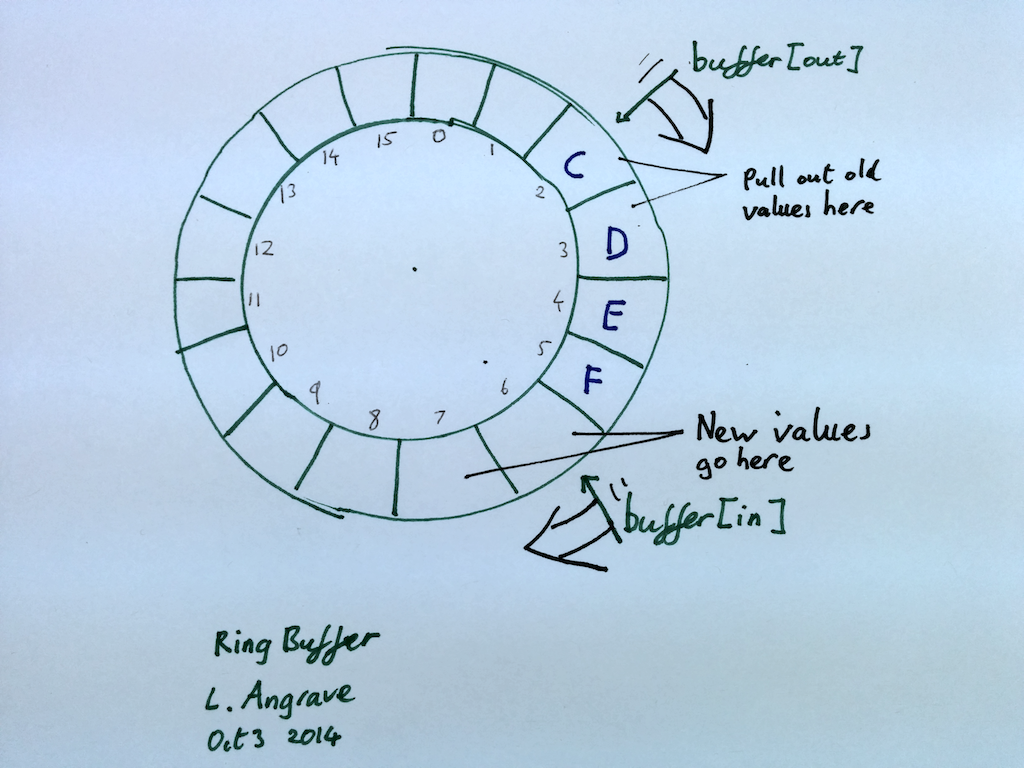
\includegraphics[width=.5\textwidth]{synchronization/images/ring_buffer.png}
\end{center}

A simple (single-threaded) implementation is shown below. Note enqueue and dequeue do not guard against underflow or overflow - it's possible to add an item when when the queue is full and possible to remove an item when the queue is empty. For example if we added 20 integers (1,2,3\ldots{}) to the queue and did not dequeue any items then values \keyword{17,18,19,20} would overwrite the \keyword{1,2,3,4}. We won't fix this problem right now, instead when we create the multi-threaded version we will ensure enqueue-ing and dequeue-ing threads are blocked while the ring buffer is full or empty respectively.

\begin{lstlisting}[language=C]
void *buffer[16];
int in = 0, out = 0;

void enqueue(void *value) { /* Add one item to the front of the queue*/
  buffer[in] = value;
  in++; /* Advance the index for next time */
  if (in == 16) in = 0; /* Wrap around! */
}

void *dequeue() { /* Remove one item to the end of the queue.*/
  void *result = buffer[out];
  out++;
  if (out == 16) out = 0;
  return result;
}
\end{lstlisting}

\subsection{What are gotchas of implementing a Ring Buffer?}\label{what-are-gotchas-of-implementing-a-ring-buffer}

It's very tempting to write the enqueue or dequeue method in the following compact form (N is the capacity of the buffer e.g.~16):

\begin{lstlisting}[language=C]
void enqueue(void *value)
  b[ (in++) % N ] = value;
}
\end{lstlisting}

This method would appear to work (pass simple tests etc) but contains a subtle bug. With enough enqueue operations (a bit more than two billion) the int value of \keyword{in} will overflow and become negative! The modulo (or `remainder') operator \keyword{\%} preserves the sign. Thus you might end up writing into \keyword{b[-14]} for example!

A compact form is correct uses bit masking provided N is 2\^{}x (16,32,64,\ldots{})

\begin{lstlisting}[language=C]
b[ (in++) & (N-1) ] = value;
\end{lstlisting}

This buffer does not yet prevent buffer underflow or overflow. For that, we'll turn to our multi-threaded attempt that will block a thread until there is space or there is at least one item to remove.


\subsection{Multithreaded Correctness}\label{checking-a-multi-threaded-implementation-for-correctness-example-1}

The following code is an incorrect implementation. What will happen? Will \keyword{enqueue} and/or \keyword{dequeue} block? Is mutual exclusion satisfied? Can the buffer underflow? Can the buffer overflow? For clarity \keyword{pthread\_mutex} is shortened to \keyword{p\_m} and we assume sem\_wait cannot be interrupted.

\begin{lstlisting}[language=C]
#define N 16
void *b[N]
int in = 0, out = 0
p_m_t lock
sem_t s1,s2
void init() { 
    p_m_init(&lock, NULL)
    sem_init(&s1, 0, 16)
    sem_init(&s2, 0, 0)
}

enqueue(void *value) {
    p_m_lock(&lock)

    // Hint: Wait while zero. Decrement and return
    sem_wait( &s1 ) 
 
    b[ (in++) & (N-1) ] = value

    // Hint: Increment. Will wake up a waiting thread 
    sem_post(&s1) 
    p_m_unlock(&lock)
}
void *dequeue(){
    p_m_lock(&lock)
    sem_wait(&s2)
    void *result = b[(out++) & (N-1) ]
    sem_post(&s2)
    p_m_unlock(&lock)
    return result
}
\end{lstlisting}

\subsection{Analysis}\label{analysis}

Before reading on, see how many mistakes you can find. Then determine what would happen if threads called the enqueue and dequeue methods.

\begin{itemize}
\tightlist
\item
  The enqueue method waits and posts on the same semaphore (s1) and similarly with equeue and (s2) i.e.~we decrement the value and then immediately increment the value, so by the end of the function the semaphore value is unchanged!
\item
  The initial value of s1 is 16, so the semaphore will never be reduced to zero - enqueue will not block if the ring buffer is full - so overflow is possible.
\item
  The initial value of s2 is zero, so calls to dequeue will always block and never return!
\item
  The order of mutex lock and sem\_wait will need to be swapped (however this example is so broken that this bug has no effect!) \#\# Checking a multi-threaded implementation for correctness (Example 1)
\end{itemize}

The following code is an incorrect implementation. What will happen? Will \keyword{enqueue} and/or \keyword{dequeue} block? Is mutual exclusion satisfied? Can the buffer underflow? Can the buffer overflow? For clarity \keyword{pthread\_mutex} is shortened to \keyword{p\_m} and we assume sem\_wait cannot be interrupted.

\begin{lstlisting}[language=C]
void *b[16]
int in = 0, out = 0
p_m_t lock
sem_t s1, s2
void init() {
    sem_init(&s1,0,16)
    sem_init(&s2,0,0)
}

enqueue(void *value){

 sem_wait(&s2)
 p_m_lock(&lock)

 b[ (in++) & (N-1) ] = value

 p_m_unlock(&lock)
 sem_post(&s1)
}

void *dequeue(){
  sem_wait(&s1)
  p_m_lock(&lock)
  void *result = b[(out++) & 15]
  p_m_unlock(&lock)
  sem_post(&s2)

  return result;
}
\end{lstlisting}

\subsubsection{Analysis}\label{analysis-1}

\begin{itemize}
\tightlist
\item
  The initial value of s2 is 0. Thus enqueue will block on the first call to sem\_wait even though the buffer is empty!
\item
  The initial value of s1 is 16. Thus dequeue will not block on the first call to sem\_wait even though the buffer is empty - oops Underflow! The dequeue method will return invalid data.
\item
  The code does not satisfy Mutual Exclusion; two threads can modify \keyword{in} or \keyword{out} at the same time! The code appears to use mutex lock. Unfortunately the lock was never initialized with \keyword{pthread\_mutex\_init()} or \keyword{PTHREAD\_MUTEX\_INITIALIZER} - so the lock may not work (\keyword{pthread\_mutex\_lock} may simply do nothing)
\end{itemize}

\subsection{Correct implementation of a ring buffer}\label{correct-implementation-of-a-ring-buffer}

The pseudo-code (\keyword{pthread\_mutex} shortened to \keyword{p\_m} etc) is shown below.

As the mutex lock is stored in global (static) memory it can be initialized with \keyword{PTHREAD\_MUTEX\_INITIALIZER}.If we had allocated space for the mutex on the heap, then we would have used \keyword{pthread\_mutex\_init(ptr, NULL)}

\begin{lstlisting}[language=C]
#include <pthread.h>
#include <semaphore.h>
// N must be 2^i
#define N (16)

void *b[N]
int in = 0, out = 0
p_m_t lock = PTHREAD_MUTEX_INITIALIZER
sem_t countsem, spacesem

void init() {
  sem_init(&countsem, 0, 0)
  sem_init(&spacesem, 0, 16)
}
\end{lstlisting}

The enqueue method is shown below. Notice: * The lock is only held during the critical section (access to the data structure). * A complete implementation would need to guard against early returns from \keyword{sem\_wait} due to POSIX signals.

\begin{lstlisting}[language=C]
enqueue(void *value){
 // wait if there is no space left:
 sem_wait( &spacesem )

 p_m_lock(&lock)
 b[ (in++) & (N-1) ] = value
 p_m_unlock(&lock)

 // increment the count of the number of items
 sem_post(&countsem)
}
\end{lstlisting}

The \keyword{dequeue} implementation is shown below. Notice the symmetry of the synchronization calls to \keyword{enqueue}. In both cases the functions first wait if the count of spaces or count of items is zero.

\begin{lstlisting}[language=C]
void *dequeue(){
  // Wait if there are no items in the buffer
  sem_wait(&countsem)

  p_m_lock(&lock)
  void *result = b[(out++) & (N-1)]
  p_m_unlock(&lock)

  // Increment the count of the number of spaces
  sem_post(&spacesem)

  return result
}
\end{lstlisting}

\subsection{Food for thought}\label{food-for-thought}

\begin{itemize}
\tightlist
\item
  What would happen if the order of \keyword{pthread\_mutex\_unlock} and \keyword{sem\_post} calls were swapped?
\item
  What would happen if the order of \keyword{sem\_wait} and \keyword{pthread\_mutex\_lock} calls were swapped?
\end{itemize}


\section{Extra: Process Synchronization}\label{process-synchronization}

You thought that you were using different processes, so you don't have to synchronize? Think again! You may not have race conditions within a process but what if your process needs to interact with the system around it? Let's consider a motivating example

\begin{lstlisting}[language=C]
void write_string(const char *data) {
    int fd = open("my_file.txt", O_WRONLY);
    write(fd, data, strlen(data));
    close(fd);
}

int main() {
    if(!fork()) {
        write_string("key1: value1");
        wait(NULL);
    } else {
        write_string("key2: value2");
    }
    return 0;
}
\end{lstlisting}

If none of the system calls fail then we should get something that looks like this (given the file was empty to begin with).

\begin{lstlisting}
key1: value1
key2: value2
\end{lstlisting}

or

\begin{lstlisting}
key2: value2
key1: value1
\end{lstlisting}

\subsection{Interruption}\label{interruption}

But, there is a hidden nuance. Most system calls can be \keyword{interrupted} meaning that the operating system can stop an ongoing system call because it needs to stop the process. So barring \keyword{fork} \keyword{wait} \keyword{open} and \keyword{close} from failing -- they typically go to completion -- what happens if \keyword{write} fails? If write fails and no bytes are written, we can get something like \keyword{key1: value1} or \keyword{key2: value2}. This is data loss which is incorrect but won't corrupt the file. What happens if write gets interrupted after a partial write? We get all sorts of madness. For example,

\begin{lstlisting}
key2: key1: value1
\end{lstlisting}

\subsection{Solution}\label{solution}

So what should we do? We should use a shared mutex! Consider the following code.

\begin{lstlisting}[language=C]
pthread_mutex_t * mutex = NULL;
pthread_mutexattr_t attr;

void write_string(const char *data) {
    pthread_mutex_lock(mutex);
    int fd = open("my_file.txt", O_WRONLY);
    int bytes_to_write = strlen(data), written = 0;
    while(written < bytes_to_write) {
        written += write(fd, data + written, bytes_to_write - written);
    }
    close(fd);
    pthread_mutex_unlock(mutex);
}

int main() {
    pthread_mutexattr_init(&attr);
    pthread_mutexattr_setpshared(&attr, PTHREAD_PROCESS_SHARED);
    pmutex = mmap (NULL, sizeof(pthread_mutex_t), 
                PROT_READ|PROT_WRITE, MAP_SHARED|MAP_ANON, -1, 0);
    pthread_mutex_init(pmutex, &attrmutex);
    if(!fork()) {
        write_string("key1: value1");
        wait(NULL);
        pthread_mutex_destroy(pmutex);
        pthread_mutexattr_destroy(&attrmutex); 
        munmap((void *)pmutex, sizeof(*pmutex));
    } else {
        write_string("key2: value2");
    }
    return 0;
}
\end{lstlisting}

What the code does in main is initialize a process shared mutex using a piece of \keyword{shared} memory. You will find out what this call to \keyword{mmap} does later -- just assume for the time being that it create memory that is shared between processes. We can initialize a \keyword{pthread\_mutex\_t} in that special piece of memory and use it as normal. To counter \keyword{write} failing, we have put the \keyword{write} call inside a while loop that keeps writing so long as there are bytes left to write. Now if all the other system calls function, there should be more more race conditions.

Most programs try to avoid this problem entirely by writing to separate files, but it is good to know that there are mutexes across processes, and they are useful. You can use all of the primitives that you were taught previously! Barriers, semaphores, and condition variables can all be initialized on a shared piece of memory and used in similar ways to their multithreading counterparts. You don't need to know the implementation, just need to know that mutexes and other synchronization primitives can be shared across processes and some of the benefits.

\begin{itemize}
\tightlist
\item
  You don't have to worry about arbitrary memory addresses becoming race condition candidates. This means that only areas that you specifically \keyword{mmap} or outside system resources like files are ever in danger.
\item
  You get the nice isolation of a processes so if one process fails the system can maintain intact
\item
  When you have a lot of threads, creating a process might ease the system load
\end{itemize}

\section{Extra: Higher Order Models of Synchronization}

When using atomics, you need to specify the right model of synchronization in order to make sure you have the correct behavior for your program.

\subsection{Sequentially Consistent}

Sequentially consistent is the simplest, least error prone and most expensive model. This model says that any change that happens, all changes before it will be synchronized between all threads.

\begin{verbatim}
    -Thread 1-              -Thread 2-
    y = 1                   if (atomic_load(x) == 2)
    atomic_store(x, 2);         y != 1 && *NULL = 1;
\end{verbatim}

Will never segfault. This is because either the store happens before the if statement in thread 2 and y == 1 or the store happens after and x does not equal 2.

\subsection{Relaxed}

\todo{Relaxed}

\subsection{Acquire/Relaxed}

\todo{Acquire/Relaxed}

\subsection{Consume}

\todo{Consume}

Examples were adapted from
\link{https://gcc.gnu.org/wiki/Atomic/GCCMM/AtomicSync}

\section{External Resources}

\begin{itemize}
\item \href{http://linux.die.net/man/3/pthread_mutex_lock}{pthread\_mutex\_lock man page} 
\item \href{http://linux.die.net/man/3/pthread_mutex_unlock}{pthread\_mutex\_unlock man page} 
\item \href{http://linux.die.net/man/3/pthread_mutex_init}{pthread\_mutex\_init man page} 
\item \href{http://linux.die.net/man/3/pthread_mutex_destroy}{pthread\_mutex\_destroy man page}
\item \href{http://man7.org/linux/man-pages/man3/sem_init.3.html}{sem\_init} 
\item \href{http://man7.org/linux/man-pages/man3/sem_wait.3.html}{sem\_wait} 
\item \href{http://man7.org/linux/man-pages/man3/sem_post.3.html}{sem\_post} 
\item \href{http://man7.org/linux/man-pages/man3/sem_destroy.3.html}{sem\_destroy}
\end{itemize}


\section{Topics}\label{topics}

\begin{itemize}
\tightlist
\item
  Atomic operations
\item
  Critical Section
\item
  Producer Consumer Problem
\item
  Using Condition Variables
\item
  Using Counting Semaphore
\item
  Implementing a barrier
\item
  Implementing a ring buffer
\item
  Using pthread\_mutex
\item
  Implementing producer consumer
\item
  Analyzing multi-threaded coded
\end{itemize}

\section{Questions}\label{questions}

\begin{itemize}
\tightlist
\item
  What is atomic operation?
\item
  Why will the following not work in parallel code

\begin{lstlisting}[language=C]
//In the global section
size_t a;
//In pthread function
for(int i = 0; i < 100000000; i++) a++;
\end{lstlisting}

  And this will?

\begin{lstlisting}[language=C]
//In the global section
atomic_size_t a;
//In pthread function
for(int i = 0; i < 100000000; i++) atomic_fetch_add(a, 1);
\end{lstlisting}
\item
  What are some downsides to atomic operations? What would be faster: keeping a local variable or many atomic operations?
\item
  What is the critical section?
\item
  Once you have identified a critical section, what is one way of assuring that only one thread will be in the section at a time?
\item
  Identify the critical section here

\begin{lstlisting}[language=C]
struct linked_list;
struct node;
void add_linked_list(linked_list *ll, void* elem){
    node* packaged = new_node(elem);
    if(ll->head){
         ll->head = 
    }else{
         packaged->next = ll->head;
         ll->head = packaged;
         ll->size++;
    }
    
}

void* pop_elem(linked_list *ll, size_t index){
    if(index >= ll->size) return NULL;
    
    node *i, *prev;
    for(i = ll->head; i && index; i = i->next, index--){
        prev = i;
    }

    //i points to the element we need to pop, prev before
    if(prev->next) prev->next = prev->next->next;
    ll->size--;
    void* elem = i->elem;
    destroy_node(i);
    return elem;
}
\end{lstlisting}

\item How tight can you make the critical section? 
\item What is a producer consumer problem? How might the above be a producer consumer problem be used in the above section? How is a producer consumer problem related to a reader writer problem? 
\item What is a condition variable? Why is there an advantage to using one over a \keyword{while} loop? 
\item Why is this code dangerous?

\begin{lstlisting}[language=C]
if(not_ready){
     pthread_cond_wait(&cv, &mtx);
}
\end{lstlisting}

\item
  What is a counting semaphore? Give me an analogy to a cookie jar/pizza box/limited food item.
\item
  What is a thread barrier?
\item
  Use a counting semaphore to implement a barrier.
\item
  Write up a Producer/Consumer queue, How about a producer consumer stack?
\item
  Give me an implementation of a reader-writer lock with condition variables, make a struct with whatever you need, it just needs to be able to support the following functions

\begin{lstlisting}[language=C]
void reader_lock(rw_lock_t* lck);
void writer_lock(rw_lock_t* lck);
void reader_unlock(rw_lock_t* lck);
void writer_unlock(rw_lock_t* lck);
\end{lstlisting}

  The only specification is that in between \keyword{reader\_lock} and \keyword{reader\_unlock}, no writers can write. In between the writer locks, only one writer may be writing at a time.
\item
  Write code to implement a producer consumer using ONLY three counting semaphores. Assume there can be more than one thread calling enqueue and dequeue. Determine the initial value of each semaphore.
\item
  Write code to implement a producer consumer using condition variables and a mutex. Assume there can be more than one thread calling enqueue and dequeue.
\item
  Use CVs to implement add(unsigned int) and subtract(unsigned int) blocking functions that never allow the global value to be greater than 100.
\item
  Use CVs to implement a barrier for 15 threads.
\item
  How many of the following statements are true?
\item
There can be multiple active readers
\item
There can be multiple active writers
\item
When there is an active writer the number of active readers must be zero
\item
If there is an active reader the number of active writers must be zero
\item
A writer must wait until the current active readers have finished
\item
  Todo: Analyzing mulithreaded code snippets
\end{itemize}

\bibliographystyle{plainnat}
\bibliography{synchronization/synchronization}
